\section{Problem Statement}


\subsection{Context and Motivation}

Large language models (LLMs) have demonstrated remarkable capabilities in understanding and generating human language, owing to their pre-training on vast corpora of textual data~\cite{brown2020language,devlin2019bert}. These models encode substantial factual and common sense knowledge within their parameters, enabling them to perform various downstream tasks ranging from question answering to content generation. However, a fundamental limitation of LLMs is that their knowledge becomes static once pre-training concludes. As the real world evolves continuously, with new discoveries, updated facts, and changing circumstances, the knowledge embedded in pre-trained models inevitably becomes outdated or incorrect.

Consider a practical scenario: an LLM trained in early 2022 would correctly answer that Nur-Sultan is the capital of Kazakhstan but would be unaware that the city was renamed back to Astana in late 2022. Similarly, models trained before the end of 2022 would not recognize information about recent events, new scientific discoveries, or updated statistics. This obsolescence of knowledge poses significant challenges for the deployment of LLMs in production environments where accuracy and currentness are critical.

The traditional approach to updating model knowledge is to perform full retraining or fine-tuning on datasets that include the new information~\cite{chung2024scaling}. However, this approach suffers from several critical drawbacks. First, retraining LLMs with billions of parameters is computationally prohibitive, requiring extensive computational resources and time that make frequent updates impractical. Second, naive fine-tuning often introduces unintended side effects: it can degrade the model's performance on tasks or knowledge domains unrelated to the update, a phenomenon known as catastrophic forgetting~\cite{luo2025empirical}. Third, fine-tuning lacks precision - it is difficult to target specific factual updates without affecting broader model behaviors. These limitations motivate the need for more surgical and efficient approaches to knowledge updating.

\begin{figure}[h]
    \centering
    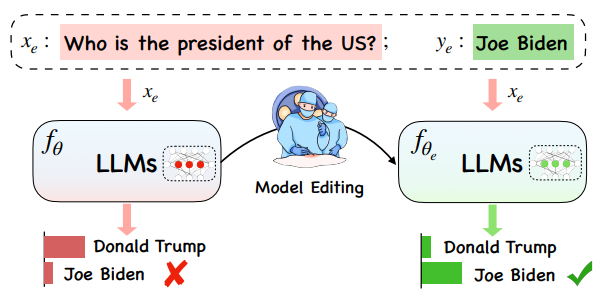
\includegraphics[width=0.7\textwidth]{figures/c1/kme_example.png}
    \caption{An example of KME for efficient update of knowledge in LLMs.}
    \label{fig:kme_example}
\end{figure}

Knowledge-based Model Editing (KME) has emerged as a promising paradigm to address these challenges~\cite{wang2024knowledge,yao2023editing}. The core principle of KME is to make precise, targeted modifications to a model's behavior on specific knowledge items while preserving its performance on unrelated inputs. Rather than retraining the entire model, KME methods aim to identify and modify the specific parameters or representations responsible for storing particular facts, enabling efficient updates without catastrophic forgetting. This approach offers the potential for practical, scalable knowledge maintenance in deployed LLMs.


\subsection{The Lifelong Model Editing Setting}

While early research in model editing focused on single, isolated edits~\cite{de2021editing,mitchell2021fast}, real-world applications demand a more challenging capability: the ability to apply a continuous stream of edits over time. This is termed \textbf{lifelong} or \textbf{continual} model editing, which is the primary focus of this report.

In the lifelong setting, the system operates in a sequential manner: at each time step $t$, it receives a new edit $e_t$ describing a knowledge update to be applied. After incorporating this edit, the model must satisfy multiple objectives simultaneously: (1) it should correctly reflect the new knowledge specified by $e_t$, (2) it should retain all previously applied edits $e_1, e_2, \ldots, e_{t-1}$, and (3) it should preserve its original behavior on knowledge unrelated to any edit. This combination of requirements makes lifelong editing substantially more challenging than single-edit scenarios.

More importantly, the lifelong setting in this report does \textbf{not} assume that all future edits are known in advance. That distinction matters because several strong methods achieve their best behavior in batch settings, where multiple edits can be optimized jointly. In contrast, the sequential protocol used in this work is intended to expose the interference and cumulative degradation that arise when updates arrive incrementally over time. Throughout this report, unless explicitly stated otherwise, ``model editing'' refers to this sequential single-fact paradigm, and evaluation is conducted incrementally across the edit stream rather than only after all edits are applied.


\subsection{Knowledge Representation and Edit Definition}

Following established conventions in the knowledge editing literature~\cite{wang2024knowledge,meng2022mass,meng2022locating,fang2024alphaedit,liu2025edit}, the report adopts a structured representation based on knowledge graph triples to formalize the model editing problem.

A unit of factual knowledge is represented as a triple $t = (s, r, o)$, where $s$ denotes the \textbf{subject}, or the entity about which information is stated, $r$ denotes the \textbf{relation}, or the type of connection or attribute being queried, and $o$ denotes the \textbf{object}, or the value that completes the statement.

Given this representation, an \textbf{edit} is defined as a transformation from an original triple to a target triple. Formally, an edit $e$ is specified by:
\begin{equation}
e = (t, t^*) = (s, r, o \rightarrow o^*),
\end{equation}
where $t = (s, r, o)$ is the original (obsolete) knowledge triple, and $t^* = (s, r, o^*)$ is the target (updated) triple. The subject $s$ and relation $r$ remain fixed, while the object changes from $o$ to $o^*$. This formulation captures the semantics of updating a particular fact: we are changing what the model believes about the relation $r$ for subject $s$.


\subsection{Input and Output Spaces}

To query a language model, a knowledge triple must be realized as natural language. This apparently simple conversion has two important consequences. First, one fact can be expressed by several surface forms, ranging from a single canonical edit prompt to multiple paraphrases that preserve the same semantics. Second, the effect of an edit is not limited to prompts that mention the edited fact directly. Once the object value of a fact is changed, prompts whose answers logically depend on that fact may also need to change, while unrelated prompts should remain stable.

For that reason, the input space of a lifelong editor must be defined more carefully than a single prompt-response pair. The thesis adopts a three-way partition that separates direct factual access, downstream logical dependence, and unaffected behavior.

\subsubsection{Three-way Input Partition}

For an edit $e = (s, r, o \rightarrow o^*)$, we partition the entire input space $\mathcal{X}$ into 3 disjoint sets:

\paragraph{1. In-Scope Inputs $\mathcal{X}_e$:} The set of natural language prompts that query the edited fact itself, including the original edit prompt and its semantically equivalent paraphrases:
\begin{equation}
\mathcal{X}_e = I(s, r) = \{x \mid x \text{ queries the value of } r(s)\}.
\end{equation}

This set is intentionally broader than a single prompt template. It includes the original surface form used to apply the edit and the alternative phrasings that should still return the same revised object once the edit is successful.

\paragraph{2. Ripple-Effect Inputs $\mathcal{R}_e$:} The set of prompts that do not directly query $(s,r)$ but whose correct answers depend on the value of $r(s)$ through multi-hop reasoning or compositional relations:
\begin{equation}
\mathcal{R}_e = \{x \mid x \text{ queries a fact logically dependent on } r(s)\}.
\end{equation}

These inputs capture the propagation behavior of an edit. They correspond to questions whose answers should change only because the edited fact has changed, not because they themselves were directly targeted.

\paragraph{3. Out-of-Scope Inputs $\mathcal{O}_e$:} The set of prompts that are semantically and logically independent of the edit:
\begin{equation}
\mathcal{O}_e = \{x \mid x \text{ is unrelated to } (s,r) \text{ and its logical consequences}\}.
\end{equation}

This set represents the region in which the editor should behave conservatively. Any broad change to this region indicates that the edit is no longer localized.

\subsubsection{Output Spaces}

Corresponding to the input spaces, we define the output spaces for each edit:

\paragraph{Original Output Space $\mathcal{Y}_e$:} Contains all acceptable natural language expressions of the original object $o$ for in-scope queries:
\begin{equation}
\mathcal{Y}_e = O(s, r, o) = \{y \mid y \text{ expresses } o \text{ as answer to } r(s)\}.
\end{equation}

\paragraph{Target Output Space $\mathcal{Y}_e^*$:} Contains the corresponding expressions of the updated object $o^*$ for in-scope queries:
\begin{equation}
\mathcal{Y}_e^* = O^*(s, r, o^*) = \{y^* \mid y^* \text{ expresses } o^* \text{ as answer to } r(s)\}.
\end{equation}

\paragraph{Ripple-Effect Target Outputs $\mathcal{Y}_e^{\text{ripple}}$:} For each prompt $x \in \mathcal{R}_e$, there exists an updated answer that logically follows from $o^*$. We denote this as $y^{\text{ripple}}(x, o^*)$, which may differ across ripple-effect queries because different downstream questions expose different logical consequences of the same factual change.

For a collection of edits $\mathcal{E} = \{e_1, e_2, \ldots, e_T\}$, we define the unions:
\begin{equation}
\mathcal{X}_{\mathcal{E}} = \bigcup_{e \in \mathcal{E}} \mathcal{X}_e, \quad
\mathcal{R}_{\mathcal{E}} = \bigcup_{e \in \mathcal{E}} \mathcal{R}_e, \quad
\mathcal{O}_{\mathcal{E}} = \bigcap_{e \in \mathcal{E}} \mathcal{O}_e.
\end{equation}

Note that $\mathcal{O}_{\mathcal{E}}$ is an intersection. An input is only out-of-scope for the full edit set if it remains unrelated to every edit that has been applied so far. This matters in the lifelong setting because a prompt that is unrelated to one edit may become relevant once several edits have accumulated.


\subsection{Formal Problem Formulation}

Let $f_\phi : \mathcal{X} \rightarrow \mathcal{Y}$ denote a pre-trained language model parameterized by $\phi \in \mathbb{R}^d$, where $\mathcal{X}$ is the space of all possible text inputs and $\mathcal{Y}$ is the space of possible outputs. Given a sequence of edits $\mathcal{E} = \{e_1, e_2, \ldots, e_T\}$ arriving over time, our goal is to produce an edited model $f_{\phi^*} : \mathcal{X} \rightarrow \mathcal{Y}^*$ with updated parameters $\phi^*$.

The objective of lifelong knowledge-based model editing is to find parameters $\phi^*$ that satisfy three requirements across all edits. The first is successful rewriting on in-scope prompts. The second is propagation to ripple-effect prompts that depend on the revised fact. The third is preservation of behavior on out-of-scope prompts. These requirements can be summarized in the following compact formulation:
\begin{equation}
\label{eq:kme_objective}
\begin{aligned}
\min_{\phi^*} \quad & \mathbb{E}_{e \sim \mathcal{E}} \Big[
    \underbrace{\mathbb{E}_{x \sim \mathcal{X}_e, \, y^* \sim \mathcal{Y}_e^*} \mathcal{L}(f_{\phi^*}(x), y^*)}_{\text{in-scope factual rewriting}}
    + \underbrace{\mathbb{E}_{x \sim \mathcal{R}_e} \mathcal{L}(f_{\phi^*}(x), y^{\text{ripple}}(x, o^*))}_{\text{ripple-effect propagation}}
    \Big], \\
\text{subject to} \quad & \underbrace{f_{\phi^*}(x) = f_\phi(x), \quad \forall x \in \mathcal{O}_{\mathcal{E}}}_{\text{locality constraint}},
\end{aligned}
\end{equation}
where $\mathcal{L}$ is a loss function, such as cross-entropy for generation, and $\phi^* = M(f_\phi; \mathcal{E})$ denotes the result of applying editing method $M$ to the original model.

This formulation is intentionally broader than a single exact-match notion of editing. The first expectation is taken over all in-scope prompts, which includes both the original edit prompt and its paraphrases. In the empirical evaluation later in the thesis, these two aspects are reported jointly as one headline metric called \textit{success}. The second expectation captures portability through ripple-effect behavior, and the constraint captures locality.

\paragraph{In-Scope Success:} The model must correctly produce target outputs $y^* \in \mathcal{Y}_e^*$ when queried with in-scope inputs $x \in \mathcal{X}_e$. Because $\mathcal{X}_e$ includes both the direct edit prompt and paraphrased variants, success is not merely prompt memorization. It is evidence that the revised fact remains usable across multiple surface forms.

\paragraph{Ripple-Effect Propagation:} The model should produce logically consistent answers for ripple-effect queries $x \in \mathcal{R}_e$.

\paragraph{Locality:} The model's behavior on out-of-scope inputs $x \in \mathcal{O}_{\mathcal{E}}$ must remain unchanged from the original model $f_\phi$. In practice, perfect preservation is unattainable because parameter updates inevitably alter internal representations to some degree. The operational question is therefore not whether any collateral effect exists, but whether such effects remain small enough to preserve unrelated behavior.

For sequential editing across time steps $t = 1, 2, \ldots, T$, the objective becomes:
\begin{equation}
f_\phi^{(t)} = M(f_\phi^{(t-1)}; e_t), \quad \text{where } f_\phi^{(0)} = f_\phi,
\end{equation}
with the requirement that at each step $t$, the edited model $f_\phi^{(t)}$ continues to satisfy Equation~\ref{eq:kme_objective} with respect to all edits applied so far: $\mathcal{E}_t = \{e_1, \ldots, e_t\}$. This is the source of the main difficulty in lifelong editing. The model is not judged only on the newest update, but on the cumulative state that remains after repeated interventions.
